% Standalone Figure 1: horizontal matched-yield audit protocol.
% The main solid path carries evidence to a per-claim verdict; the two controls
% stay on a separate dashed bus and are not deployable action recommendations.
% Compile: make fig0_overview.pdf  (see Makefile)
\documentclass[11pt,tikz,border=2pt]{standalone}
\usepackage[T1]{fontenc}
\usepackage{amsmath,amssymb}
\usepackage{newtxtext}
\usepackage{newtxmath}
\usetikzlibrary{arrows.meta,calc,positioning}

\definecolor{FAblue}{HTML}{0072B2}
\definecolor{FAaqua}{HTML}{009E73}
\definecolor{FAorange}{HTML}{E69F00}
\definecolor{FAviolet}{HTML}{CC79A7}
\definecolor{FAred}{HTML}{D55E00}
\definecolor{FAyellow}{HTML}{F0E442}
\definecolor{FAink}{HTML}{0B0B0B}
\definecolor{FAinktwo}{HTML}{333333}
\definecolor{FAtick}{HTML}{666666}
\definecolor{FAgrid}{HTML}{E1E0D9}
\definecolor{FAsurface}{HTML}{FCFCFB}

\newcommand{\accentbar}[2]{%
  \fill[#2] ([xshift=0.7mm,yshift=-1.2mm]#1.north west)
    rectangle ([xshift=2.1mm,yshift=1.2mm]#1.south west);}
\newcommand{\cylinder}[2]{%
  \begin{scope}[shift={(#1,#2)},draw=FAblue,line width=0.65pt]
    \draw (-3.0mm,2.1mm) arc (180:360:3.0mm and 0.85mm);
    \draw (-3.0mm,-2.1mm) -- (-3.0mm,2.1mm) (3.0mm,-2.1mm) -- (3.0mm,2.1mm);
    \draw (-3.0mm,-2.1mm) arc (180:360:3.0mm and 0.85mm);
    \draw (-3.0mm,2.1mm) arc (180:0:3.0mm and 0.85mm);
  \end{scope}}
\newcommand{\funnel}[2]{%
  \begin{scope}[shift={(#1,#2)},draw=FAaqua,line width=0.7pt]
    \draw (-3.7mm,2.6mm) -- (3.7mm,2.6mm) -- (1.1mm,-0.3mm)
      -- (1.1mm,-2.7mm) -- (-1.1mm,-2.7mm) -- (-1.1mm,-0.3mm) -- cycle;
  \end{scope}}
\newcommand{\gridicon}[2]{%
  \begin{scope}[shift={(#1,#2)},draw=FAorange,line width=0.6pt]
    \draw (-2.8mm,-2.8mm) rectangle (2.8mm,2.8mm);
    \draw (-2.8mm,0) -- (2.8mm,0) (0,-2.8mm) -- (0,2.8mm);
    \fill[FAorange!22] (-2.8mm,0) rectangle (0,2.8mm);
  \end{scope}}
\newcommand{\shield}[2]{%
  \begin{scope}[shift={(#1,#2)},draw=FAviolet,line width=0.65pt]
    \draw (-2.7mm,2.5mm) -- (2.7mm,2.5mm) -- (2.2mm,-0.8mm)
      .. controls (1.6mm,-2.2mm) and (0.6mm,-2.9mm) .. (0,-3.2mm)
      .. controls (-0.6mm,-2.9mm) and (-1.6mm,-2.2mm) .. (-2.2mm,-0.8mm) -- cycle;
    \draw[line width=0.8pt] (-1.3mm,-0.1mm) -- (-0.3mm,-1.2mm) -- (1.5mm,1.2mm);
  \end{scope}}
\newcommand{\seal}[2]{%
  \begin{scope}[shift={(#1,#2)},draw=FAyellow!85!black,line width=0.65pt]
    \draw (0,0) circle (3.0mm); \draw (0,0) circle (2.2mm);
    \draw[line width=0.8pt] (-1.4mm,0) -- (-0.3mm,-1.2mm) -- (1.6mm,1.3mm);
  \end{scope}}
\newcommand{\shuffleicon}[2]{%
  \begin{scope}[shift={(#1,#2)},draw=FAaqua,line width=0.6pt,
    >={Latex[length=1.0mm,width=0.8mm]}]
    \draw[->] (-3.0mm,1.3mm) .. controls (-0.5mm,1.3mm) and (0.5mm,-1.3mm) .. (3.0mm,-1.3mm);
    \draw[->] (-3.0mm,-1.3mm) .. controls (-0.5mm,-1.3mm) and (0.5mm,1.3mm) .. (3.0mm,1.3mm);
  \end{scope}}
\newcommand{\packicon}[2]{%
  \begin{scope}[shift={(#1,#2)},draw=FAred,line width=0.65pt]
    \draw (-2.5mm,-2.4mm) rectangle (2.5mm,1.3mm);
    \draw (-2.5mm,1.3mm) -- (0,2.8mm) -- (2.5mm,1.3mm);
    \draw[line width=0.8pt] (-1.5mm,-1.4mm) -- (1.5mm,1.4mm)
      (-1.5mm,1.4mm) -- (1.5mm,-1.4mm);
  \end{scope}}

\begin{document}
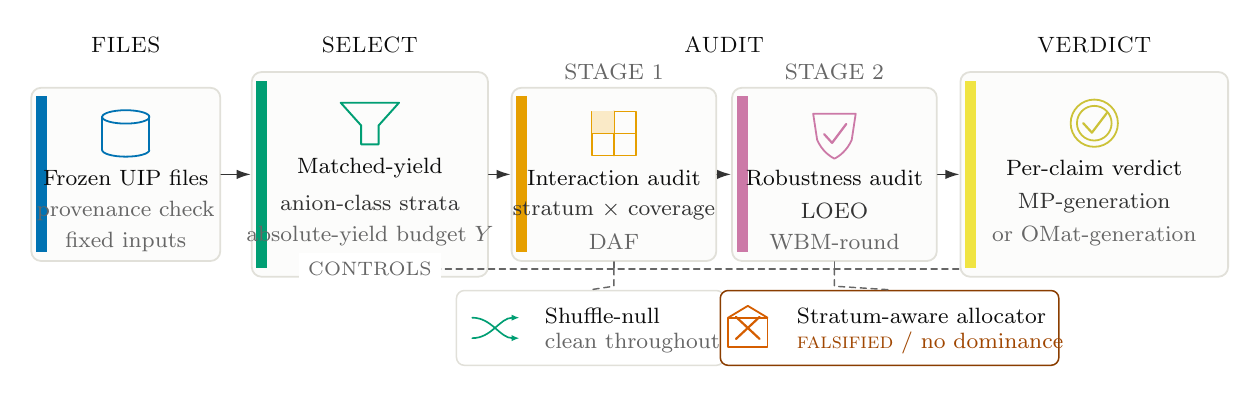
\begin{tikzpicture}[
  x=1mm,y=1mm,
  font=\rmfamily\fontsize{8.2}{9.6}\selectfont,
  line cap=round,line join=round,
  >={Latex[length=1.8mm,width=1.2mm]},
  flow/.style={draw=FAinktwo,line width=0.58pt,-{Latex[length=1.8mm,width=1.2mm]}},
  control/.style={draw=FAtick,line width=0.52pt,dash pattern=on 2.2pt off 1.7pt},
  stage/.style={draw=FAgrid,line width=0.65pt,rounded corners=1.25mm,fill=FAsurface,
    align=center,inner sep=0pt},
  chip/.style={draw=FAgrid,line width=0.55pt,rounded corners=1.0mm,fill=white,
    align=center,inner sep=0pt},
  heading/.style={font=\rmfamily\scshape\fontsize{7.8}{8.8}\selectfont,text=FAink},
  body/.style={font=\rmfamily\fontsize{7.8}{9.0}\selectfont,text=FAinktwo},
  strong/.style={font=\rmfamily\fontsize{8.4}{9.6}\selectfont,text=FAink},
  note/.style={font=\rmfamily\fontsize{7.5}{8.6}\selectfont,text=FAtick,
    fill=white,inner xsep=1.2mm,align=center}
]

% Headers. AUDIT spans the two sequential audit stages.
\node[heading] at (12,18.5) {FILES};
\node[heading] at (43,18.5) {SELECT};
\node[heading] at (88,18.5) {AUDIT};
\node[heading] at (135,18.5) {VERDICT};
\node[body,text=FAtick] at (74,15.0) {STAGE 1};
\node[body,text=FAtick] at (102,15.0) {STAGE 2};

% Solid evidence path: box height tracks content (icon + 3 text lines), no dead air.
\node[stage,minimum width=24mm,minimum height=22mm] (files) at (12,2) {};
\accentbar{files}{FAblue}
\cylinder{12}{7.2}
\node[strong] at (12,1.6) {Frozen UIP files};
\node[body,text=FAtick] at (12,-2.6) {provenance check};
\node[body,text=FAtick] at (12,-6.6) {fixed inputs};

\node[stage,minimum width=30mm,minimum height=26mm] (select) at (43,2) {};
\accentbar{select}{FAaqua}
\funnel{43}{8.5}
\node[strong] at (43,2.8) {Matched-yield};
\node[body] at (43,-1.6) {anion-class strata};
\node[body,text=FAtick] at (43,-5.8) {absolute-yield budget $Y$};

\node[stage,minimum width=26mm,minimum height=22mm] (stageone) at (74,2) {};
\accentbar{stageone}{FAorange}
\gridicon{74}{7.2}
\node[strong] at (74,1.6) {Interaction audit};
\node[body] at (74,-2.6) {stratum $\times$ coverage};
\node[body,text=FAtick] at (74,-6.6) {DAF};

\node[stage,minimum width=26mm,minimum height=22mm] (stagetwo) at (102,2) {};
\accentbar{stagetwo}{FAviolet}
\shield{102}{7.2}
\node[strong] at (102,1.6) {Robustness audit};
\node[body] at (102,-2.6) {LOEO};
\node[body,text=FAtick] at (102,-6.6) {WBM-round};

\node[stage,minimum width=34mm,minimum height=26mm] (verdict) at (135,2) {};
\accentbar{verdict}{FAyellow}
\seal{135}{8.5}
\node[strong] at (135,2.8) {Per-claim verdict};
\node[body] at (135,-1.6) {MP-generation};
\node[body,text=FAtick] at (135,-5.8) {or OMat-generation};

\draw[flow] (files.east) -- (select.west);
\draw[flow] (select.east) -- (stageone.west);
\draw[flow] (stageone.east) -- (stagetwo.west);
\draw[flow] (stagetwo.east) -- (verdict.west);

% Controls bus immediately under the stage bottoms.
\draw[control] (43,-10) -- (118,-10);
\draw[control] (stageone.south) -- (74,-10);
\draw[control] (stagetwo.south) -- (102,-10);
\node[note] at (43,-10) {CONTROLS};

\node[chip,minimum width=34mm,minimum height=9.5mm] (shuffle) at (71,-17.5) {};
\shuffleicon{59}{-17.5}
\node[strong,anchor=west] at (64,-16.0) {Shuffle-null};
\node[body,anchor=west,text=FAtick] at (64,-19.4) {clean throughout};

\node[chip,draw=FAred!65!black,minimum width=43mm,minimum height=9.5mm] (allocator) at (109,-17.5) {};
\packicon{91}{-17.5}
\node[strong,anchor=west] at (96,-16.0) {Stratum-aware allocator};
\node[body,anchor=west,text=FAred!75!black] at (96,-19.4)
  {\textsc{falsified} / no dominance};

\draw[control] (74,-10) -- (74,-12.2) -- (shuffle.north);
\draw[control] (102,-10) -- (102,-12.2) -- (allocator.north);

\end{tikzpicture}
\end{document}
